% This is text associated with the open textbook "Open Electromagnetics"
% See immediately below for author, date
% This work is licensed under the Creative Commons Attribution-ShareAlike 4.0 International License. (CC BY SA 4.0) 
% To view a copy of the license, visit http://creativecommons.org/licenses/by-sa/4.0/

%ORB TITLE Boundary Conditions on the Magnetic Flux Density ({\bf B}) 
%ORB AUTHOR 0        # S.W. Ellingson, Virginia Tech (ellingson@vt.edu)
%ORB DATE 20180806   # yyyymmdd
%ORB ABSTRACT Boundary Conditions on the Magnetic Flux Density

\label{m0022_Boundary_Conditions_on_B} % <-- Must match name of this file and module directory name.  Don't mess with this!

In homogeneous media, electromagnetic quantities vary smoothly and continuously.
At an interface between dissimilar media, however, it is possible for electromagnetic quantities to be discontinuous.
Continuities and discontinuities in fields can be described mathematically by \emph{boundary conditions} 
\index{boundary conditions}
and used to constrain solutions for fields away from these interfaces.

In this section, we derive the boundary condition on the magnetic flux density ${\bf B}$ at a smooth interface between two material regions, as shown in Figure~\ref{m0022_fBoundary}.\footnote{It may be helpful to note the similarity (duality, in fact) between this derivation and the derivation of the associated boundary condition on ${\bf D}$ presented in Section~\ref{m0021_Boundary_Conditions_on_D}.} 
%
\begin{figure}[b!]
\begin{center}
\pdftooltip{{  % note double braces
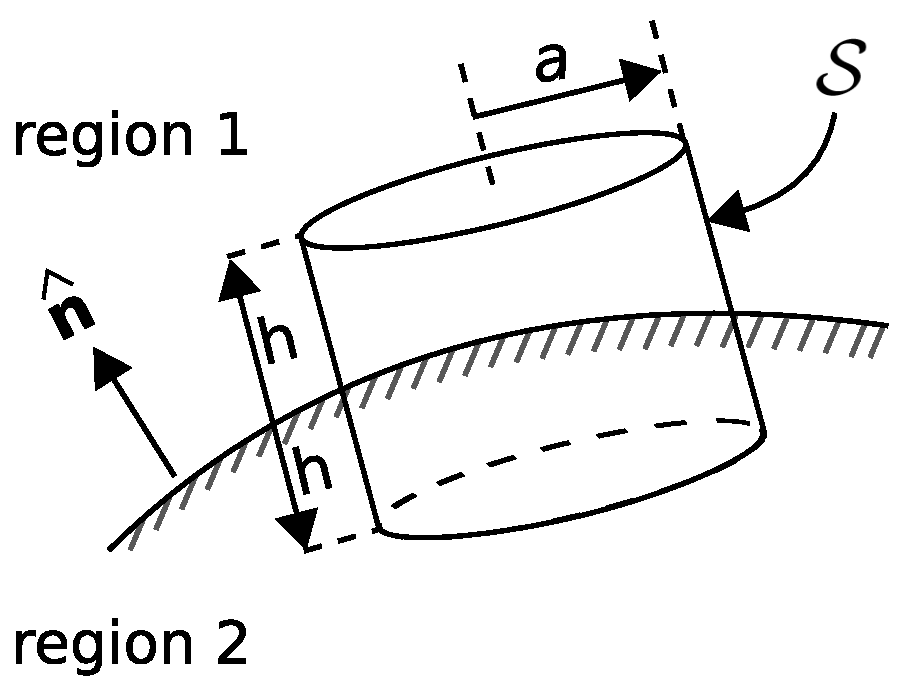
\includegraphics[width=2in]{modules/m0022_fBoundary.eps}
% https://commons.wikimedia.org/wiki/File:M0022_fBoundary.svg
}}{A closed cylinder with surface, S, is centered at a point on an interface. The flat ends are parallel to the surface and n-hat extends perpendicular to the surface. The radius of the cylinder is a, and the hight is h. The region outside the interface is labeled region 1, and the inner is labeled region 2. }
\end{center} 
\centerline{\scriptsize 
\copyright~\hyperref[m0022_fBoundary_Credit]{K.\ Kikkeri} 
\href{https://creativecommons.org/licenses/by-sa/4.0/}{CC BY~SA 4.0} 
} 
\caption{
\label{m0022_fBoundary}
Determination of the boundary condition on ${\bf B}$ at the interface between material regions.
}
\end{figure}
%
The desired boundary condition may be obtained from Gauss' Law for Magnetic Fields (GLM; Section~\ref{m0018_Gauss_Law_Magnetic_Integral_Form}):
%
\begin{equation}
\oint_{\mathcal S} {\bf B}\cdot d{\bf s} = 0
\end{equation}
%
where ${\mathcal S}$ is any closed surface.
Let ${\mathcal S}$ take the form of cylinder centered at a point on the interface, and for which the flat ends are parallel to the surface and perpendicular to $\hat{\bf n}$, as shown in Figure~\ref{m0022_fBoundary}.  
Let the radius of this cylinder be $a$, and let the length of the cylinder be $2h$.  From GLM, we have
%
\begin{align}
\oint_{\mathcal S}{ {\bf B} \cdot d{\bf s} } &= \int_{top} { {\bf B} \cdot d{\bf s} } &            \nonumber \\
                                                 &+ \int_{side} { {\bf B} \cdot d{\bf s} } &            \nonumber \\
                                                 &+ \int_{bottom} { {\bf B} \cdot d{\bf s} } &= 0
\end{align}
% 
Now let us reduce $h$ and $a$ together while (1) maintaining a constant ratio $h/a\ll 1$ and (2) keeping $\mathcal{S}$ centered on the interface.
Because $h\ll a$, the area of the side can be made negligible relative to the area of the top and bottom.
Then, as $h\to 0$, we are left with    
%
\begin{equation}
\int_{top} { {\bf B} \cdot d{\bf s} } + \int_{bottom} { {\bf B} \cdot d{\bf s} }  \to 0
\end{equation}
%
As the area of the top and bottom sides become infinitesimal, the variation in ${\bf B}$ over these areas becomes negligible.  Now we have simply:  
%
\begin{equation}
{\bf B}_1 \cdot \hat{\bf n}\Delta A + {\bf B}_2 \cdot \left( -\hat{\bf n} \right) \Delta A \to 0
\end{equation}
%
where ${\bf B}_1$ and ${\bf B}_2$ are the magnetic flux densities at the interface but in regions~1 and 2, respectively,
and $\Delta A$ is the area of the top and bottom sides.  
Note that the orientation of $\hat{\bf n}$ is important -- we have assumed $\hat{\bf n}$ points into region~1, and we must now stick with this choice.
Thus, we obtain 
%
\begin{equation}
\boxed{
\hat{\bf n} \cdot \left( {\bf B}_1 - {\bf B}_2 \right) = 0
}
\label{m0022_eBCB}
\end{equation}       
%
where, as noted above, $\hat{\bf n}$ points into region~1.

Summarizing:
%
%ORB HIGHLIGHT
\begin{mdframed}[backgroundcolor=yellow!20,nobreak=true] 
The normal (perpendicular) component of ${\bf B}$ across the boundary between two material regions is continuous.
\end{mdframed}

It is worth noting what this means for the magnetic field intensity ${\bf H}$. Since ${\bf B}=\mu{\bf H}$, it must be that
%
%ORB HIGHLIGHT
\begin{mdframed}[backgroundcolor=yellow!20,nobreak=true] 
The normal (perpendicular) component of ${\bf H}$ across the boundary between two material regions is discontinuous if the permeabilities are unequal.
\end{mdframed}




